\chapter{Experimental program: mechanical properties and performance of corroded rebars}
\label{chap-three}

Corrosion is the main aging condition that affects structures. Therefore, the success of this study relies on the most accurate representation of the corrosion process in the analytical model. As mentioned in Chapter 2, previous studies developed accelerated corrosion rebar specimens with high current densities, but did not account for the depassivation process of the reinforcing steel. A main objective of this study is to verify the mechanical properties of corroded rebars while considering the depassivation process in rebars. The experimental process is divided in to three main components, (1) generate the passive layer in rebar specimens, (2) depassivate and corrode the rebar specimens, and (3) obtain the mechanical properties of the reinforcing steel by performing tension tests and buckled bar tension (BBT) tests. It is expected that these tests will mimic as best as possible the real aging conditions of rebars inside a concrete mix. The results obtained from the tension and BBT tests will be used to update the analytical model presented in Chapter\ref{chap-four}, and more broadly provide accurate mechanical properties of corroded rebars.

\section{Proposed experimental campaign}

Rebars embedded in concrete generate a protective film that protects the rebars against corrosion, due to the alkaline environment of the cement paste. The most common form of corrosion occurs via chloride attacks. During a chloride attack, the chloride diffuses in the concrete cover and enters in contact with the surface of the rebars. This initiates the process of depassivation in which the protective film on the surface of the rebar is eliminated. The depassivation of the rebar enables the process of corrosion to occur. The proposed experimental campaign described in this chapter aims to simulate the process of corrosion as it would occur in rebars embedded in concrete. Using as received rebars, that is no special treatment to the surface of the rebar, the tests procedure consist of (1) protect the rebar ends that will be used as grips during the tension and perform buckled bar tension (BBT) tests, (2)  generate the passive layer on the rebars, (3) perform accelerated corrosion of the rebars until the specified levels of corrosion, (4) perform tension tests to characterize the tension stress-strain behavior of corroded rebars, and (5) perform the BBT tests that will provide data on the ultimate limit state of corroded rebars. The different procedures of the experimental campaign are further explained below.

\textbf{Preparation of rebar ends}

First, it is necessary to protect the areas of the rebar that are going to function as grips for the rebars during the tension and BBT tests against corrosion. Therefore, the ends of the rebars will be protected with three layers. The first layer consists of two-part epoxy, the second layer consists of electroplater tape, and the third layer consists of shrink tube. These layers will ensure minimal corrosion in the grip areas of the rebar. \fref{fig:RebarSpecimenGeomtry} and \fref{fig:RebarEndsProtection} show the specimen geometry and the protective layers at the ends of the rebars.
\begin{figure}[htbp]
	\centering
	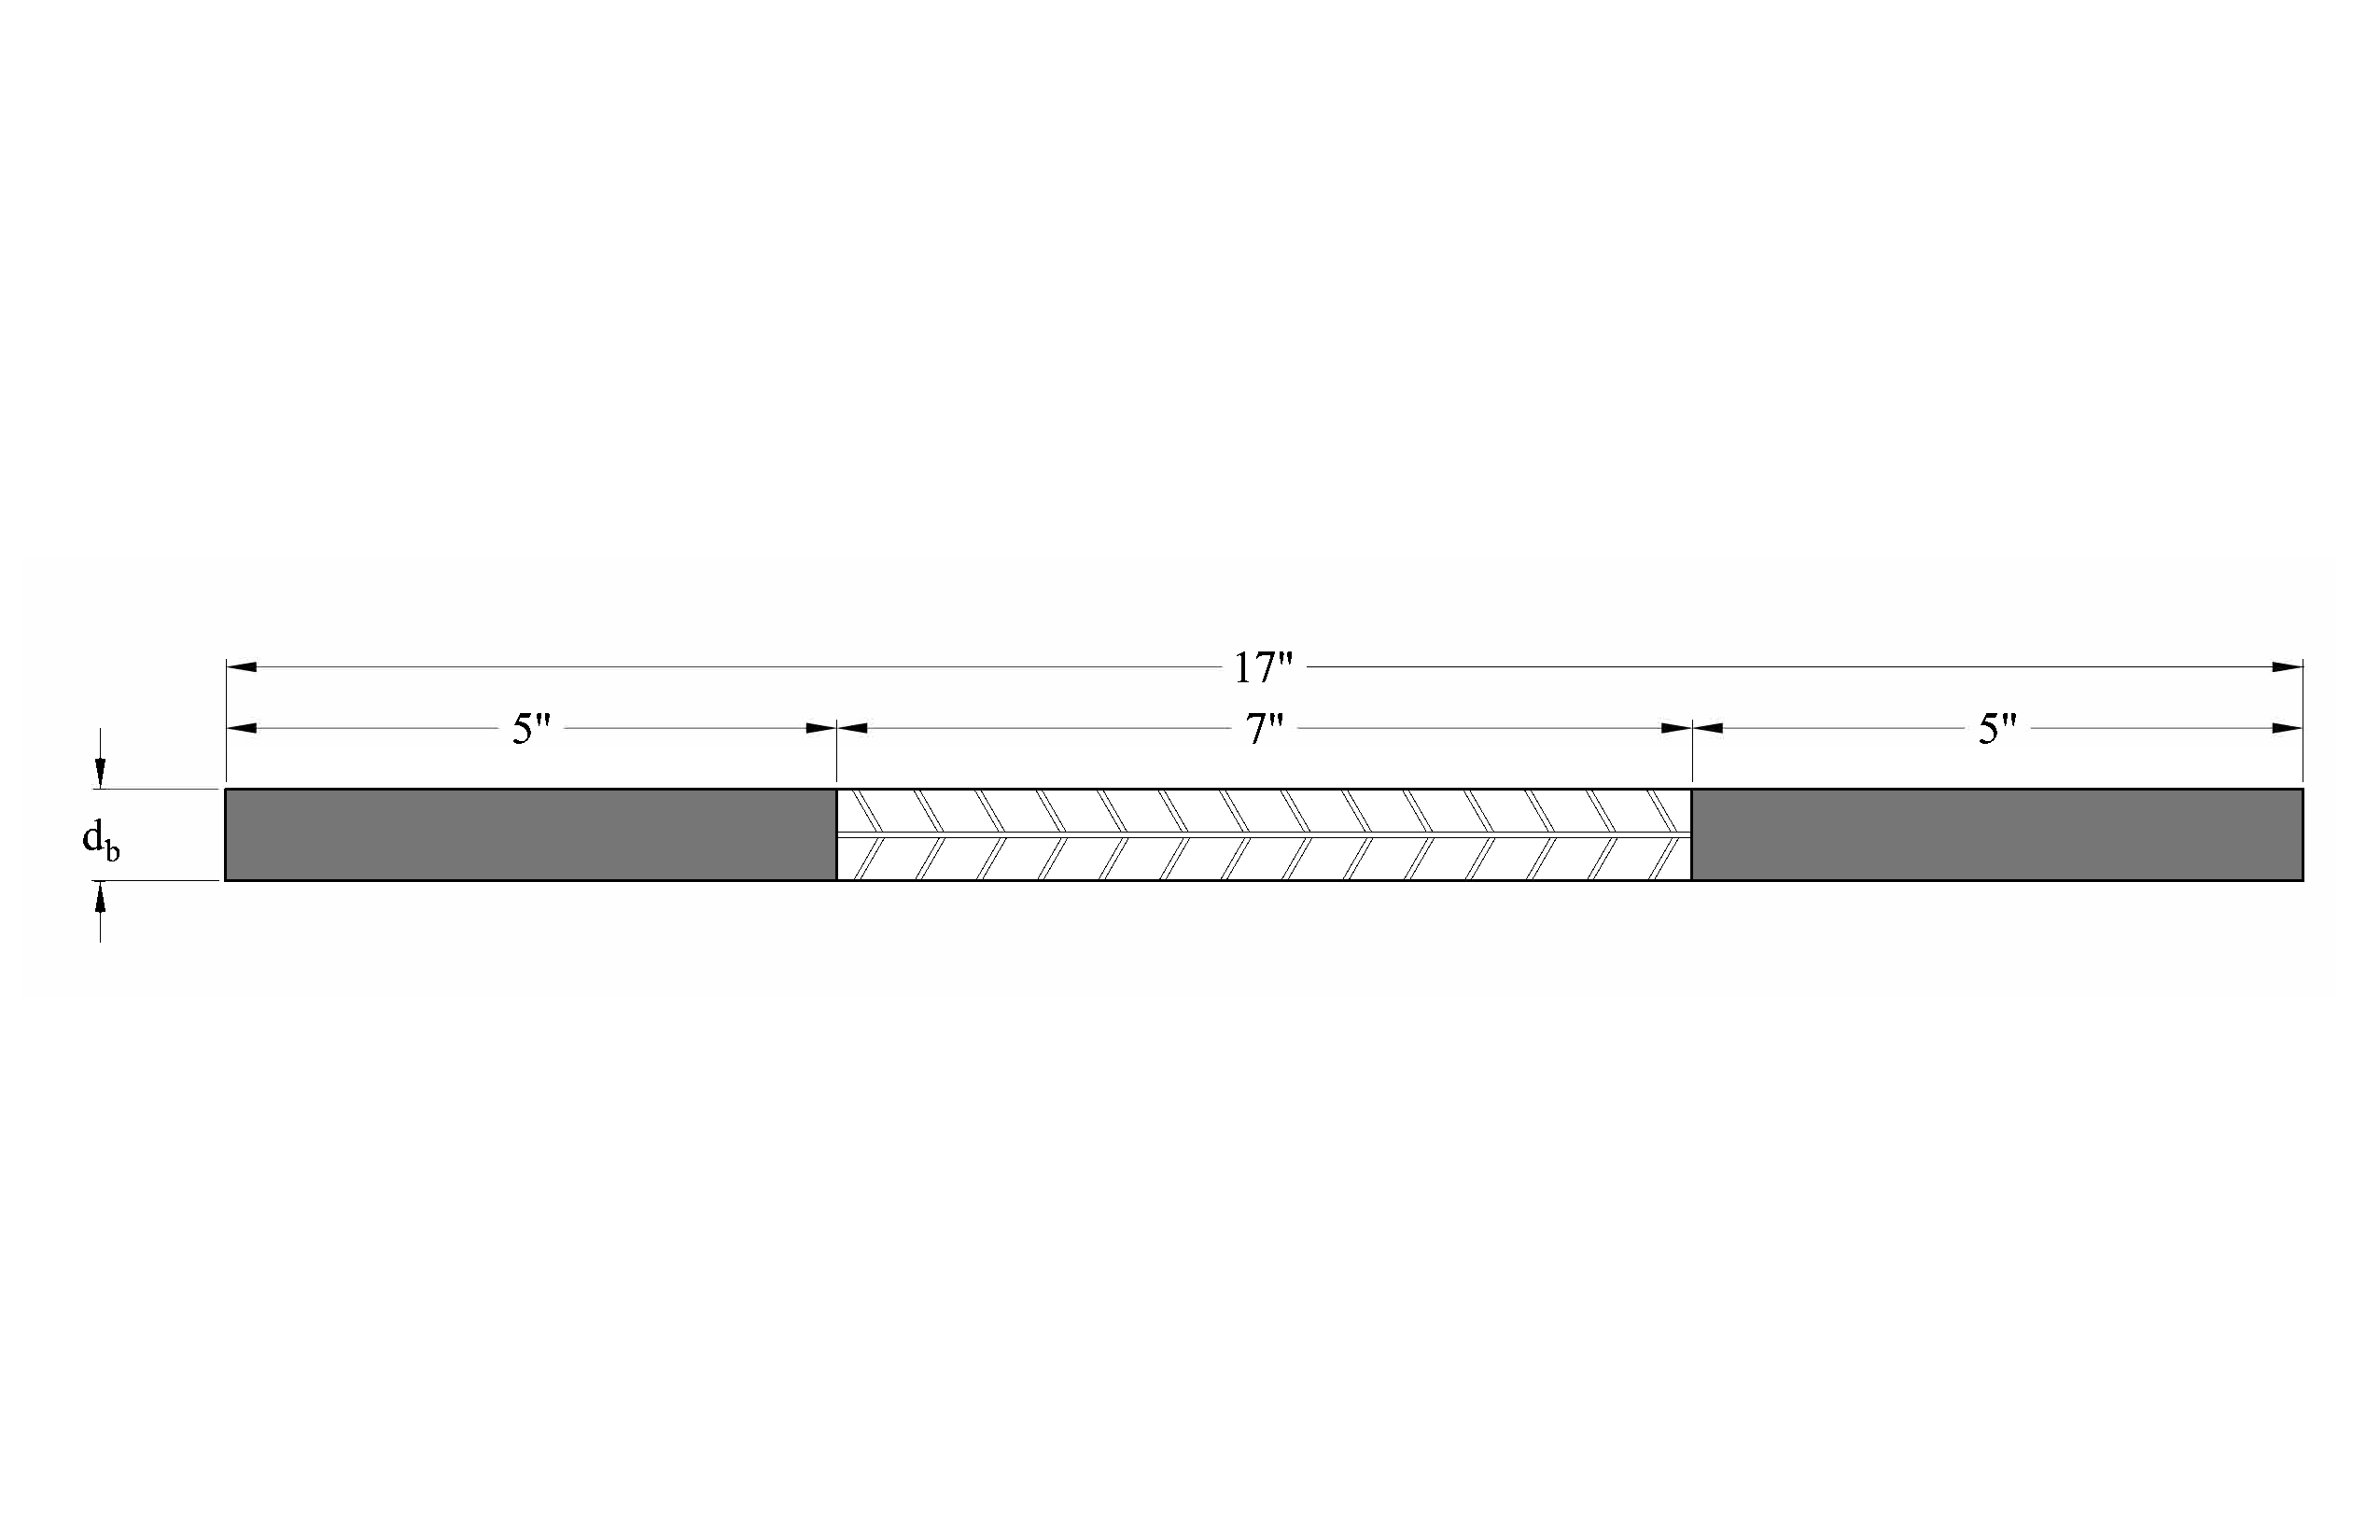
\includegraphics[width=1.0\textwidth]{Chapter-3/figs/RebarSamples}
	\caption{Rebar Specimen Geometry}
	\label{fig:RebarSpecimenGeomtry}
\end{figure}

\begin{figure}[htbp]
	\centering
	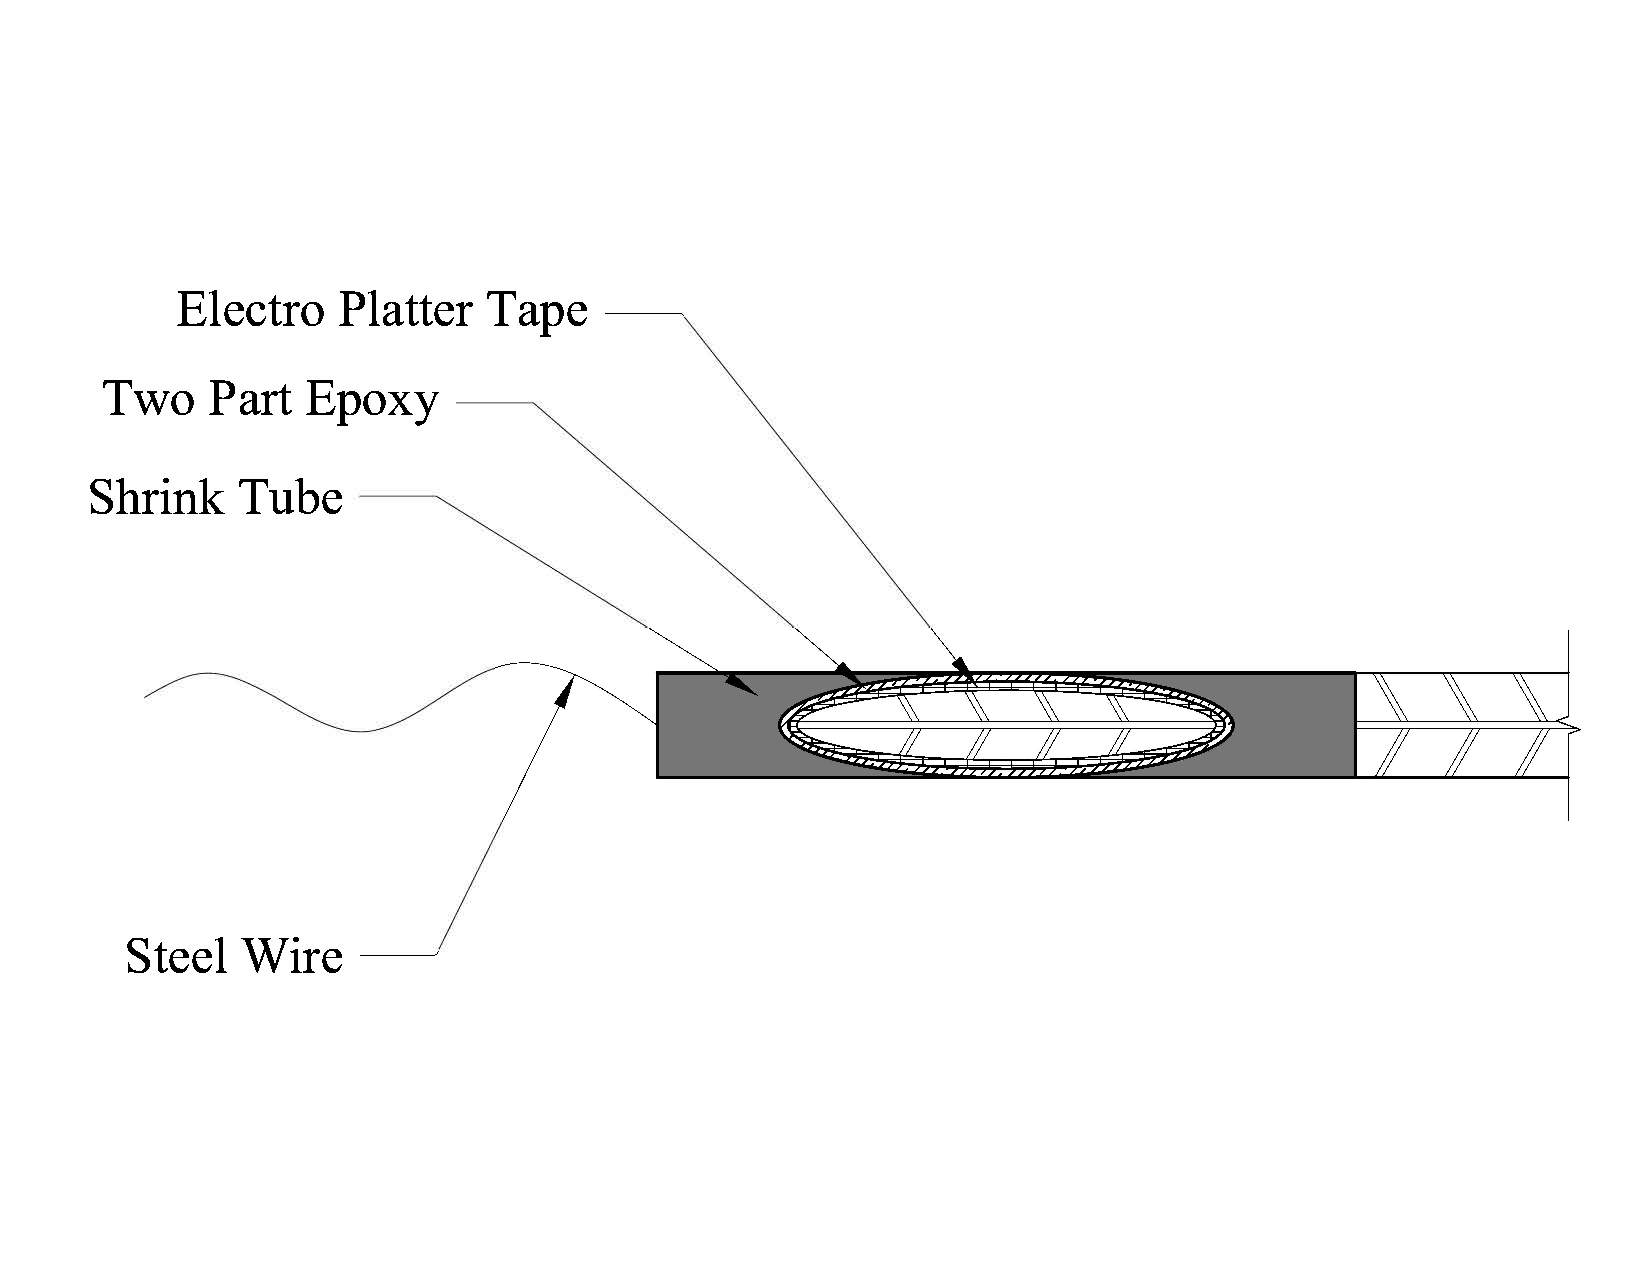
\includegraphics[width=0.7\textwidth]{Chapter-3/figs/Rebar_Ends}
	\caption{Rebars Ends Protection}
	\label{fig:RebarEndsProtection}
\end{figure}
\newpage 

To optimize the space and time it takes to prepare the rebars for corrosion, a large rebar that contains three specimens will be prepared. This ensures that the large specimen, which will be placed in a corrosion cell, provides the same level of corrosion to all the specimen subsets. After each large specimen has the specified level of corrosion, the large specimen will be cut into the three smaller specimens shown in \fref{fig:RebarSpecimenGeomtry}.

\begin{figure}[htbp]
	\centering
	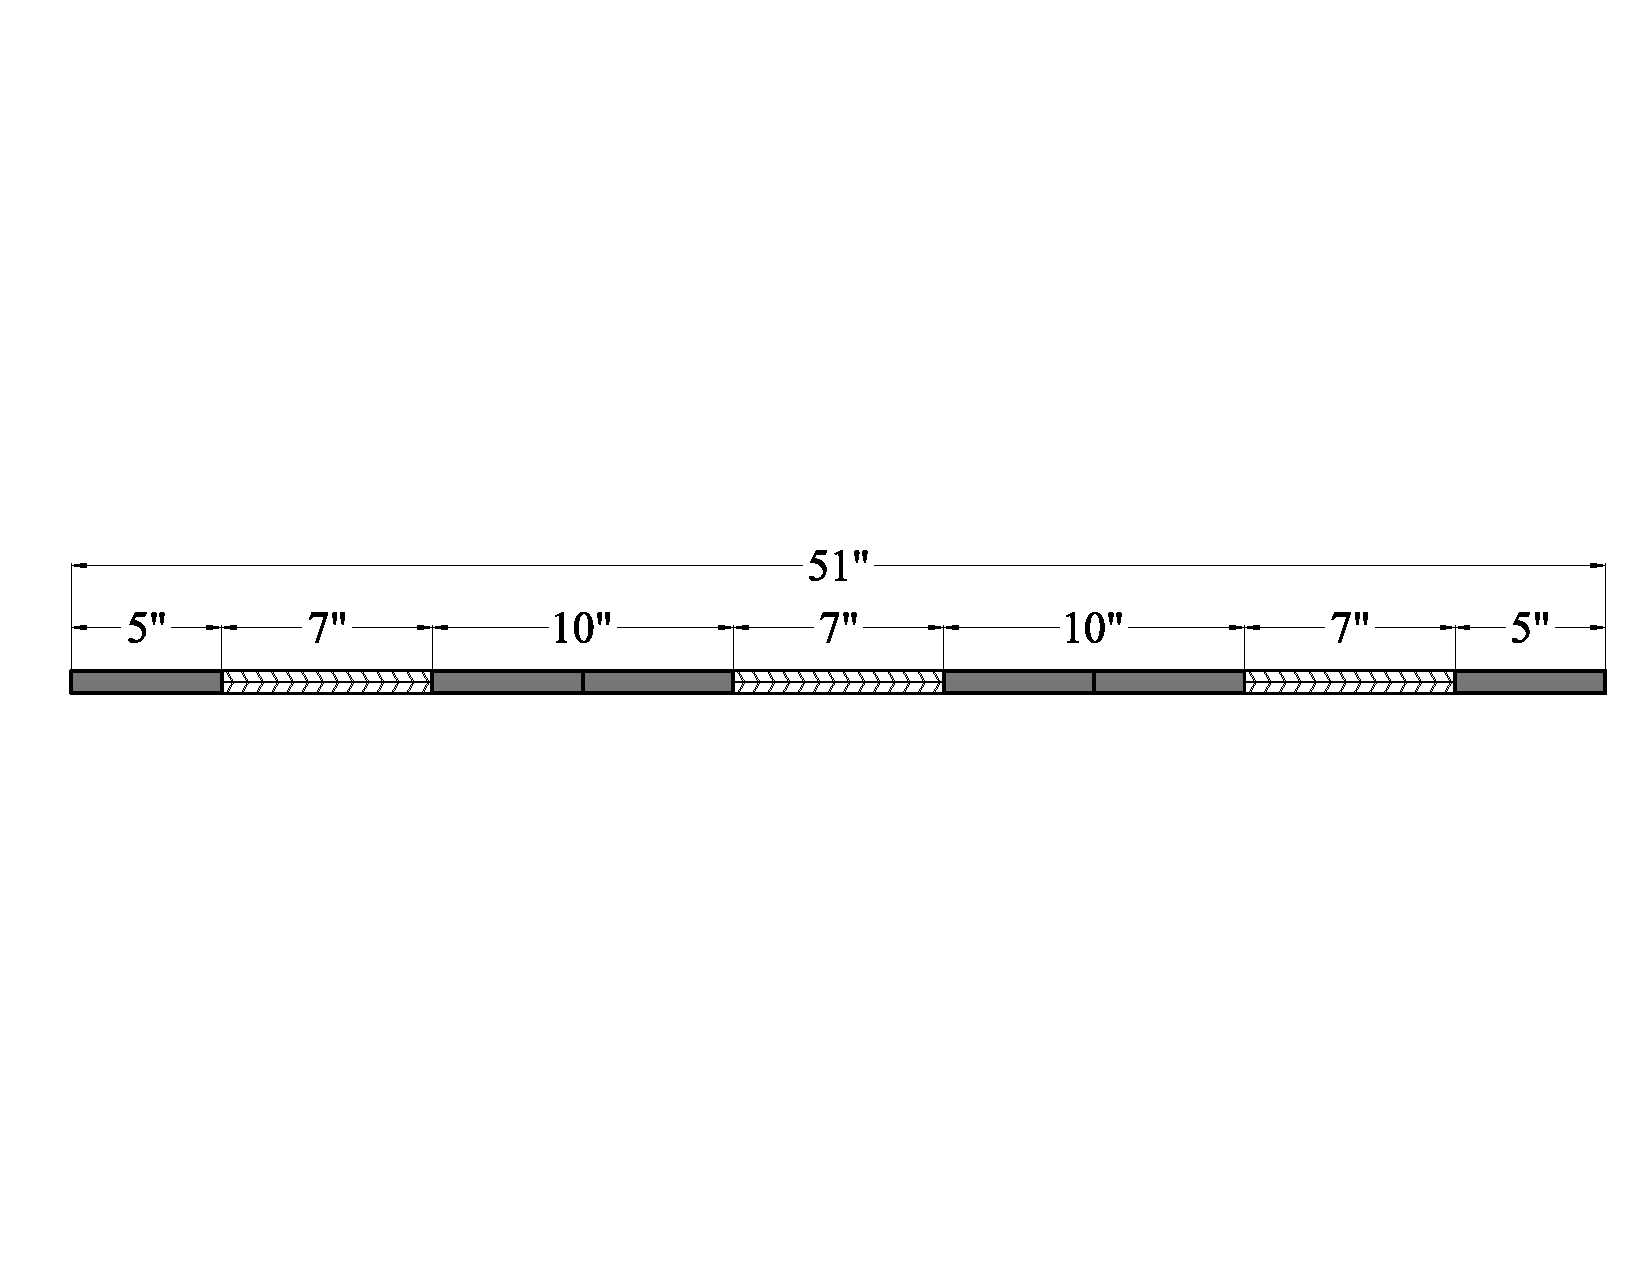
\includegraphics[width=1.0\textwidth]{Chapter-3/figs/LargeSpecimen}
	\caption{Large specimen containing three subset of specimens}
	\label{fig:LargeSpecimen}
\end{figure}

\newpage

\textbf{Passivation of the rebars}

In order to simulate the conditions of rebars embedded in concrete, it is necessary to generate the passive layer on the surface of the rebars. There are two ways to generate the passive layer: (1) embed rebars in concrete and wait for the passive layer to generate, or (2) submerge the reinforcing steel in a synthetic pore solution that mimics the cement paste environment. The second option is more suited for material testing since it does not involve demolishing the concrete. To this regard, Ghods et al \cite{Ghods2010} developed ten different pore solutions to generate the passive film on the surface of rebars. The pore solutions that were developed in their study intended to mimic the cement paste. Their study conducted 10 solutions designed to encompass concentrations of $Ca^{+2}$, $Na^{+}$, $K^{+}$, and $(SO_{4})^{+}$ found in the cement paste. The solution that generated the passive layer with the best quality of protective film will be used in this study. To achieve the desired concentration of the $Ca^{+2}$, $Na^{+}$, $K^{+}$, and $(SO_{4})^{+}$ ions, the following concentration of chemicals recommended in \cite{Ghods2010} will be used in the pore solution:

\begin{itemize}
	\item Saturated calcium hydroxide $Ca(OH)_2$ (approx. 1.7 g/L)
	\item Sodium hydroxide $Na(OH)$ (4.00 g/l)
	\item Potassium hydroxide $(KOH)$ (11.22 g/l)
	\item Calcium sulfate dehydrate $Ca(SO)_4 + 2H_2O$ (13.77 g/l)
\end{itemize}

The rebars will be placed in the pore solution as received without any special surface preparation in the area of study, since any form of special surface preparation affects the quality of the passive layer \cite{Andersson1989}, \cite{DawnMarcotte2001}, \cite{Moragues1987}, and \cite{Page1983}.In addition, Ghods et al showed that no significant change in the anodic polarization of the rebar surface after being placed in the pore solution for 8 days or 14 days. Their results are shown in \fref{fig:GhodsRebarPassivation}. Therefore the rebars will be placed in the pore solution for a minimum of 8 days. 

\begin{figure}[htbp]
	\centering
	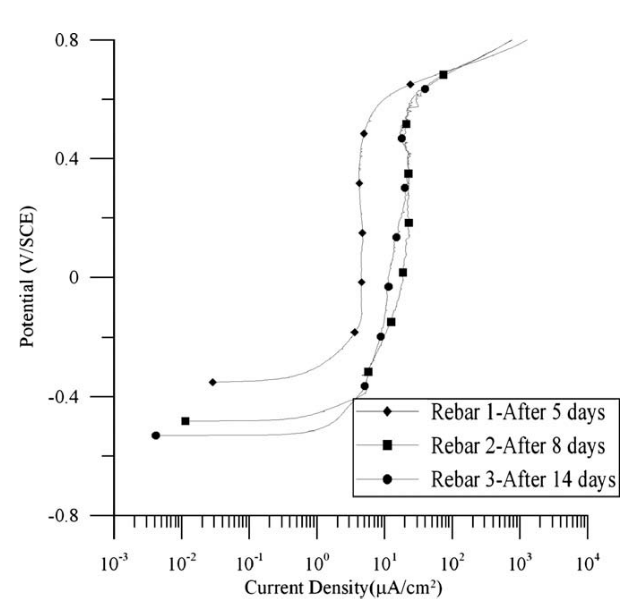
\includegraphics[width=0.6\textwidth]{Chapter-3/figs/AsReceived_AnodicPolarization_time}
	\caption{As received rebars anodic polarization immersed in pore solution for different times\cite{Ghods2009}}
	\label{fig:GhodsRebarPassivation}
\end{figure}

To prepare the rebars for the development of the passive layer, a specimen preparation assembly will be developed. The assembly consists of placing the rebar inside a PVC pipe, closing the ends of the pipe  with a $90^{\circ}$ PVC elbow, and closing the open ends with PVC pipe plugs. The assembly is shown in \fref{fig:RebarPassivation}. This assembly ensures that the pipe remains airtight and prevents the carbonation of the calcium hydroxide ($Ca(OH)_{2}$ in the pore solution.

\begin{figure}[htbp]
	\centering
	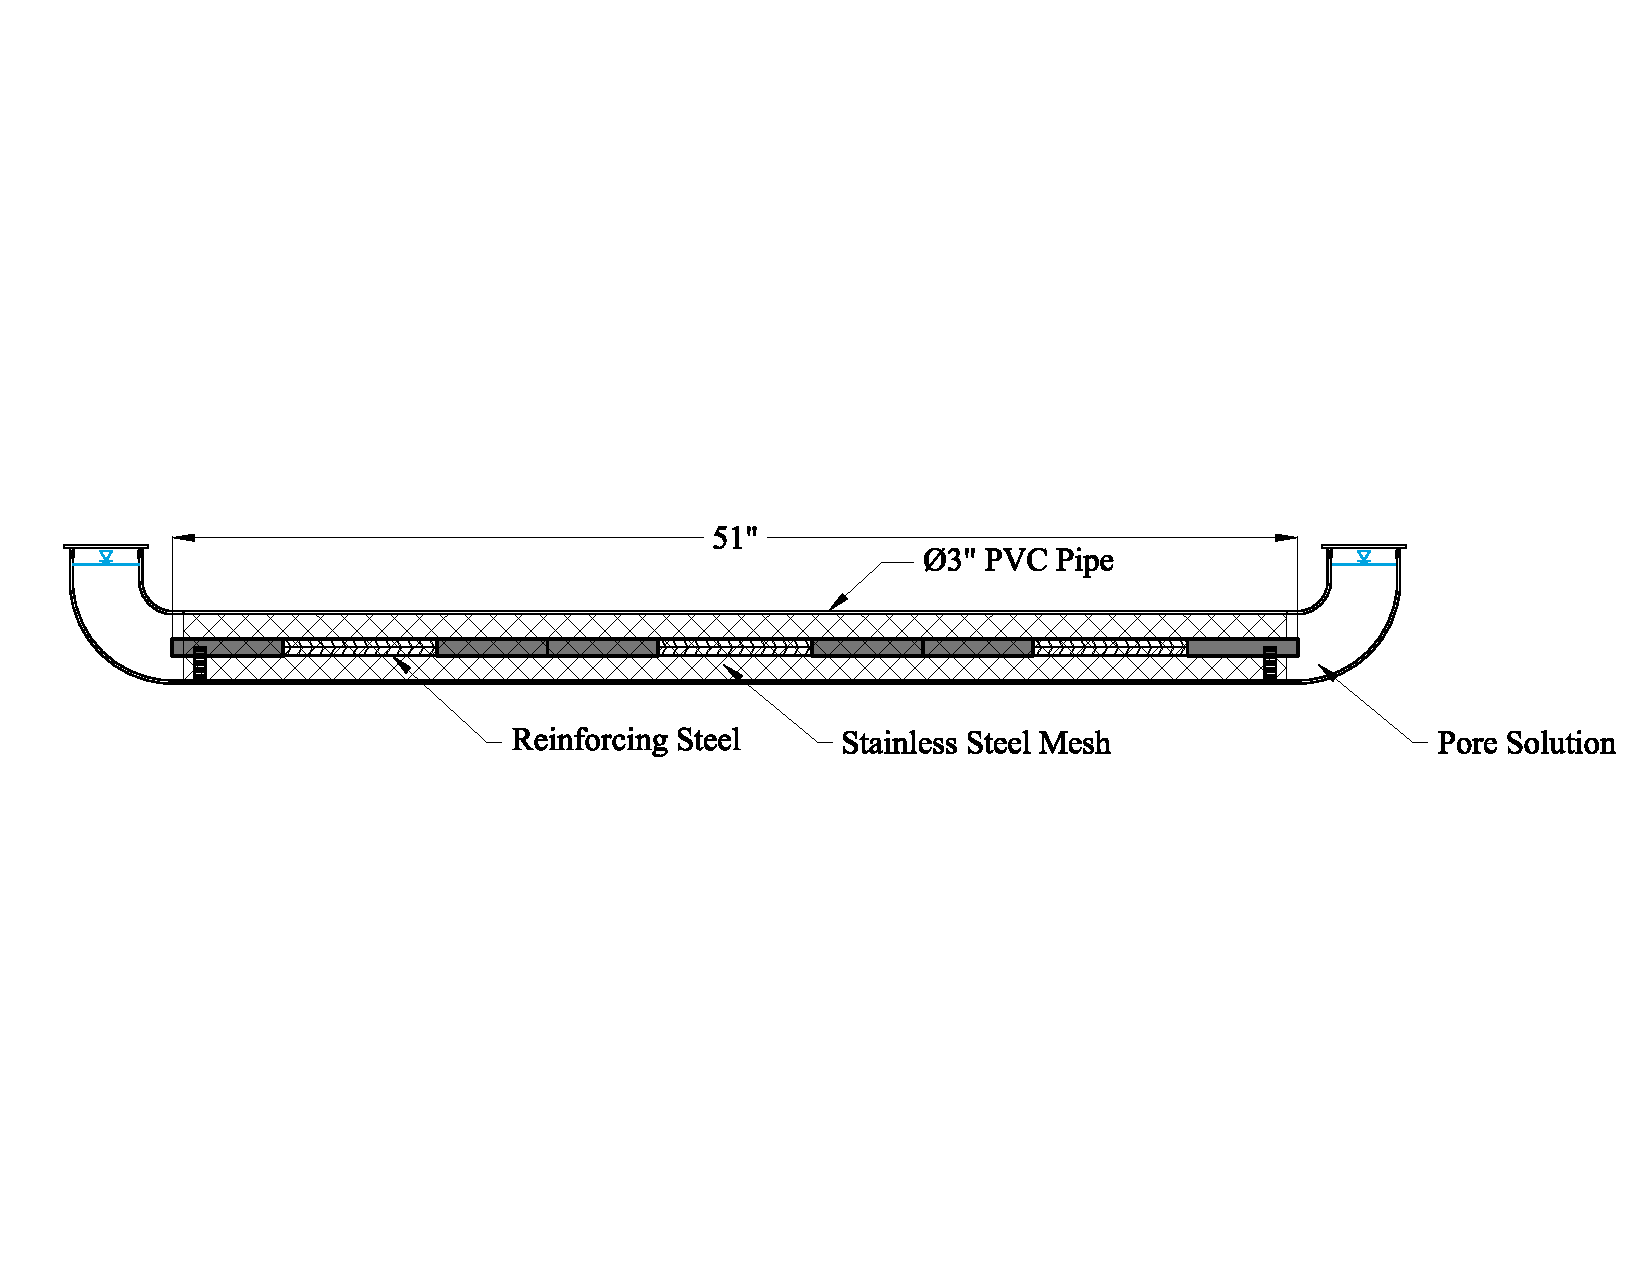
\includegraphics[width=1.0\textwidth]{Chapter-3/figs/AnodicPolarization_01}
	\caption{Assembly for rebar preparation for the development of passive layer in pore solution}
	\label{fig:RebarPassivation}
\end{figure}

\newpage
\textbf{Accelerated corrosion  of reinforcing steel}

Four components are required for corrosion to occur: (1) the anode, (2) the cathode, (3) an electrolytic connection, and (4) an electrical path. The corrosion cell that will be deployed in this study uses this concept in the following way: the anode consists of the rebar, the cathode consists of a stainless steel mesh, the electrolytic connection will be made with a sodium chloride solution, and the electrical path is forced via an electric circuit. The corrosion cell uses the assembly developed to generate the passive layer with the components needed for corrosion as shown in \fref{fig:AcceleratedCorrosion}. The circuit was designed so that the current in the specimen is $5mA$, equivalent to $47\mu A/cm^2$ on the bare surface of the rebar. Since the rebar and stainless steel mesh have a low resistance, a $1k\Omega$ resistor will be added to the circuit, such that it stabilizes the current and keeps it constant at $5mA$.

\begin{figure}[htbp]
	\centering
	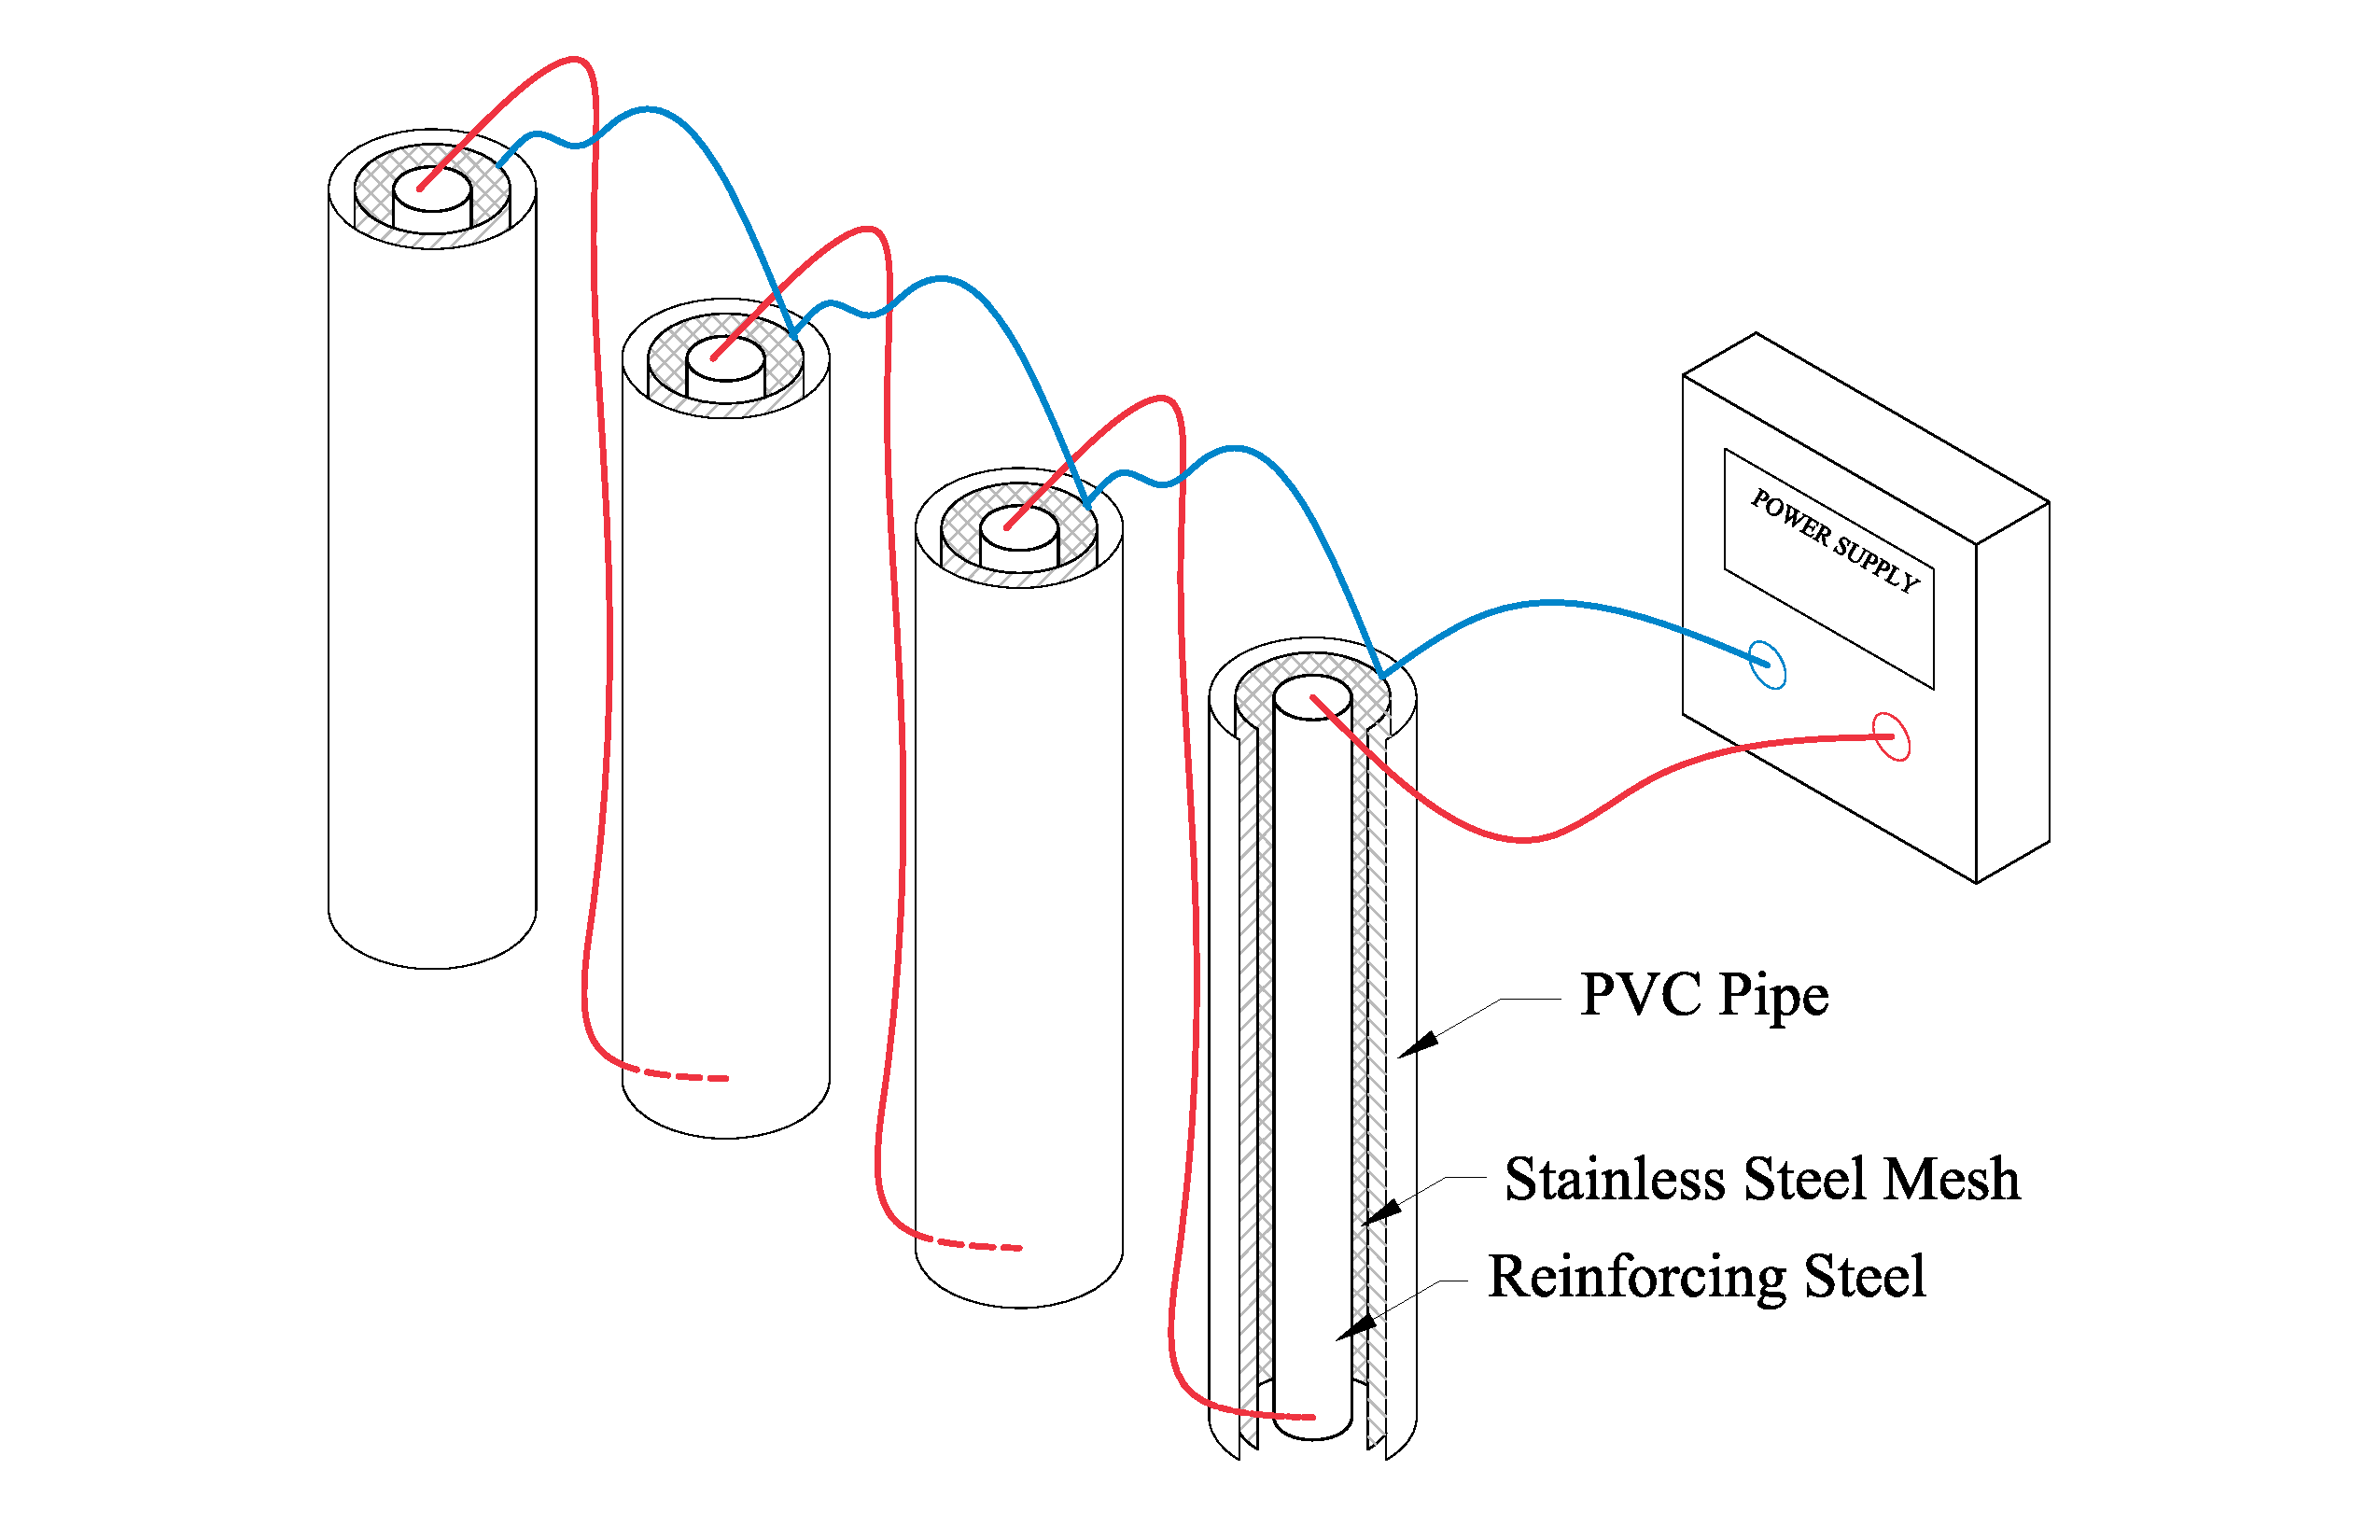
\includegraphics[width=0.95\textwidth]{Chapter-3/figs/AcceleratedCorrosionProcedure}
	\caption{Accelerated corrosion process}
	\label{fig:AcceleratedCorrosion}
\end{figure}

Ghods et al \cite{Ghods2010} determined that for rebars with passive films, a concentration of 0.3 Moles of sodium chloride ($NaCl$) will start the depassivation process on the rebars. Accordingly ithe same sodium chloride solution will be used in this study. To estimate the time to apply the current and obtain the desired level of corrosion,  Faraday's law shown in equation \ref{eq.FaradayEq} is used.

\begin{equation}
	m_{loss}=\frac{it(AM)}{nF}
	\label{eq.FaradayEq}
\end{equation}

 In equation \ref{eq.FaradayEq}, $m_{loss}$ corresponds to the mass loss, $i$ is the current in amperes ($i=5 mA$), $t$ is the time the current is sustained in seconds $(AM)$ is the atomic mass of the oxidizing component. For this study the oxidizing component is the iron ($Fe$) in the rebars, hence $(AM)=54.845g/mol$, $n$ is the number of electrons lost per atom oxidized, for $Fe$ the number of electrons is equal to 2, and $F$ is Faraday's number ($F=96485 C$). Solving \eref{eq.FaradayEq} for $t$ and assuming uniform corrosion for different corrosion levels, the time of application is calculated. The estimated times to achieve the corrosion levels is shown in Table \ref{tab:AcceleratedCorrosionTime}. 

\begin{table}[htbp]
	\caption{Accelerated corrosion times in 3/4" rebar}
	\label{tab:AcceleratedCorrosionTime}
	\centering	
		\begin{tabular}{|l|c|c|}
		\hline
		Corrosion Level (CL) & Mass loss (g)   & time (days)     \\  \hline	
		5\%                  & 0.93            & 7.5    \\  \hline	
		10\%                 & 1.86            & 15     \\  \hline	
		15\%                 & 2.80            & 22.5   \\  \hline	
		20\%                 & 3.73            & 30     \\  \hline	
		25\%                 & 5               & 37.3   \\  \hline	
		\end{tabular}
\end{table}

\textbf{Tension tests}

The tension tests will be performed to evaluate differences in the stress-strain behavior of corroded reinforcing steel with those found in the literature. In addition, the data obtained from these tests will serve as an input to the analytical model. Therefore, a series of tension tests will be performed accordingly. The tension tests will be performed in accordance with the standard ASTM A370, which specifies the loading procedure and the gauge lengths. The tension tests consist of:
\begin{enumerate}
    \item Place the rebar in the universal testing machine
    \item Pull the rebar in tension 
    \item Record the load and the strain on the rebar 
\end{enumerate}

The strains will be captured through the use of LED markers from the Optrotrak Certus HD system. The gauge length between the LED markers will be 2inches as is specified in the ASTM A370 standard, \fref{fig:TensionTest} shows an example of the test setup. The stress will be calculated based on the load reading from the UTM machine and divided by the measured area of the corroded rebars.

\begin{figure}[htbp]
	\centering
	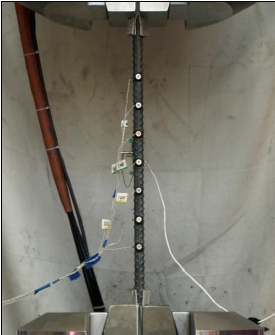
\includegraphics[width=0.4\textwidth]{Chapter-3/figs/TensionTest}
	\caption{Tension test setup example\cite{Overby2016}}
	\label{fig:TensionTest}
\end{figure}

The results obtained from the tension tests will be valuable to understand the change in the stress-strain relationship, the yield strength, and ultimate strength of corroded rebars. Statistical analysis of the results will help to update equations that correlate these parameters to the corrosion level, and potentially yield an updated form of  \eref{eq.eleven}. The outcomes of the tension tests will further improve the results of the analytical model in Chapter \ref{chap-four}.
\newline

\textbf{Buckled bar tension (BBT) test}

One of the limit states considered in the seismic design of bridge columns is the buckling of rebar. Recent tests have been developed to determine the critical bending strain of buckled reinforcing steel \cite{Barcley2019}, which is associated with the sudden fragile fracture of longitudinal reinforcement of RC column. The buckled bar tension (BBT) test simulates the bending and tension strain demands on a buckled bar to determine critical bending strain in buckled rebars. 

Barcley et al \cite{Barcley2019} developed a methodology to calculate local strains on a buckled bar using an LED optical sensor system \cite{NorthernDigitalInc.2020}. \fref{fig:BBTseq} shows the basic concept of the BBT test.

\begin{figure}[htbp]
	\centering
	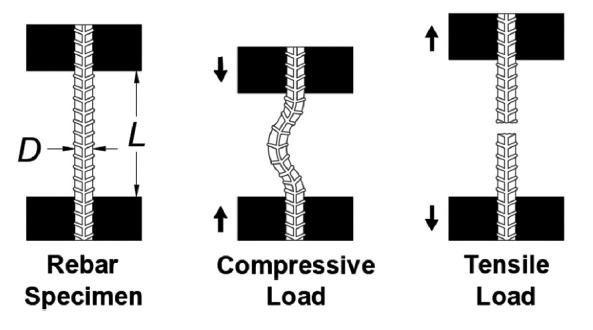
\includegraphics[width=0.7\textwidth]{Chapter-3/figs/BBT_Sequence}
	\caption{BBT Test sequence\cite{Barcley2019}}
	\label{fig:BBTseq}
\end{figure}

The procedure to perform the buckled bar tension test consists of:

\begin{enumerate}
    \item First, place rebar in a universal testing machine (UTM), and prepare the rebar specimen with LED markers on the surface of the specimen such that the displaced shape of the bar can be measured.
    \item Second, compress the rebar specimen to impose a bending strain of a prescribed level. Barcley et al showed that a fourth order polynomial can be fit to the LED sensors near the buckled region of the bar to obtain the displaced shape ($w$). The bending strain is calculated using solid mechanics principles. Curvature is the second derivative of the displaced shape ($w$) for small displacements, which is calculated as: 
    \begin{equation}
        \phi=\frac{\frac{d^2w(x)}{dx^2}}{\left[1+\left(\frac{dw(x)}{dx}\right)\right]^\frac{3}{2}}\approx \frac{d^2w(x)}{dx^2}
        \label{eq.CuvatureAprox}
    \end{equation}
    If we assume that the bending is symmetric for the rebar then the strain in the extreme fibers of the rebar is calculated as:
    \begin{equation}
        \varepsilon_{b}=\phi\left(\frac{d_{bl}}{2}\right) 
        \label{eq.BendingStrain}
    \end{equation}    
    Combining equations \eref{eq.CuvatureAprox}, and \eref{eq.BendingStrain}, the bending strain can be expressed as:
    \begin{equation}
        \varepsilon_{b}=\frac{d^2w(x)}{dx^2}\left(\frac{d_{bl}}{2}\right) 
        \label{eq.BendingStrainExpanded}
    \end{equation}
    An example of the calculation of the bending strain is shown in \fref{fig:BBT_Curvature}
    \item Third, once buckled to the prescribed curvature, the bar is loaded in tension until fracture is observed
    \item Then the process is repeated with a different bar for a different bending strain. After all the tests are performed results from elongation at peak force can be generated as the example shown in \fref{fig:BBT_MaxBendingStrain}. From the results obtained through BBT tests the critical bending strain can be determined. The critical bending strain is defined as the point at which a low elongation under load is obtained. This low elongation results in a brittle fracture of the rebar as shown in \fref{fig:BBT_DuctileBrittle}(b). \fref{fig:BBT_MaxBendingStrain} shows that for bars with rebars the critical bending strain is $\varepsilon_{b}=0.10$ for grade 80 ksi steel.
\end{enumerate}

\begin{figure}[htbp]
    \centering
    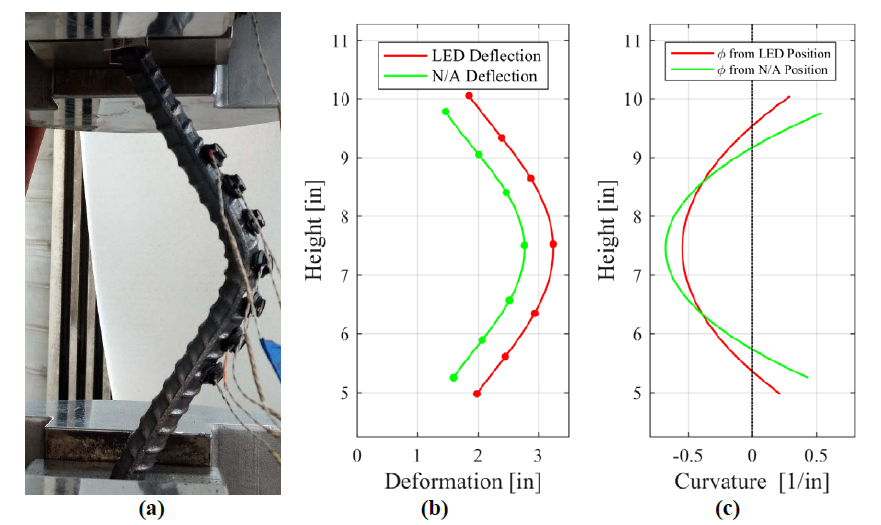
\includegraphics[width=0.8\textwidth]{Chapter-3/figs/BBT_Curvature}
    \caption{a) Picture of buckled bar; (b) Position of optical markers and adjustment to neutral axis; (c) Calculation of curvature \cite{Barcley2018}}
    \label{fig:BBT_Curvature}
\end{figure}
\begin{figure}
    \centering
    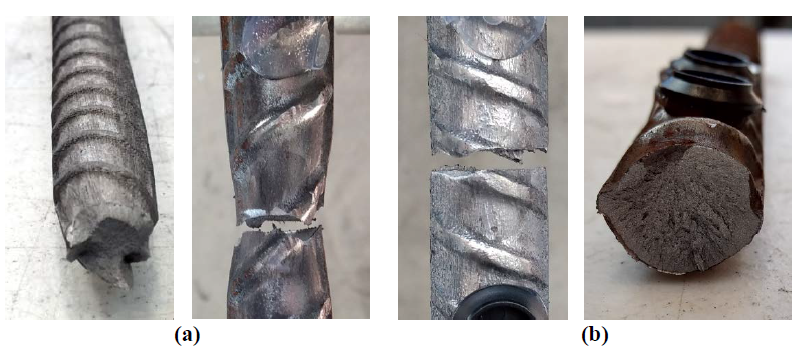
\includegraphics[width=1.0\textwidth]{Chapter-3/figs/BBT_Ductile_vs_Brittle}
    \caption{(a)Ductile rebar fracture; (b) Brittle rebar fracture \cite{Barcley2018}}
    \label{fig:BBT_DuctileBrittle}
\end{figure}
\begin{figure}[htbp]
    \centering
    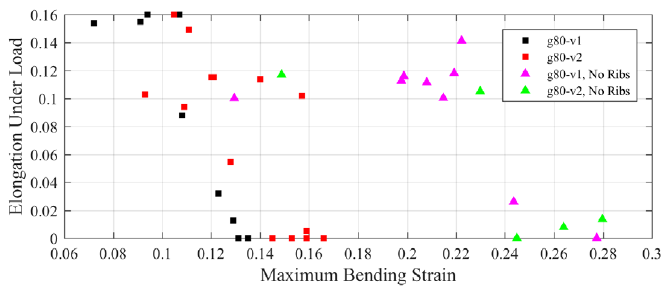
\includegraphics[width=1.0\textwidth]{Chapter-3/figs/BBT_MaxBendignStrain}
    \caption{BBT results for rebars with and without ribs \cite{Barcley2018}}
    \label{fig:BBT_MaxBendingStrain}
\end{figure}

\newpage

The BBT tests are proposed for different levels of corrosion such that any changes on the behavior are studied and incorporated in the analytical model. The proposed test matrix is shown in Table \ref{tab:Test Matrix}. It must be noted that in each corrosion level for the BBT tests, each experiment will correspond to a different prescribed bending strain. The selection for each prescribed bending strains consist of 1) Start with the maximum bending strain determined in previous research to be around $\varepsilon=0.10$ as shown in \fref{fig:BBT_MaxBendingStrain}, 2)if brittle fracture is observed the next test will be at a lower bending strain for example $\varepsilon=0.08$, 3)otherwise higher strains such as $\varepsilon=0.12$ will be evaluated. This is repeated for each corrosion level. It is expected that six tests per corrosion level will be sufficient however, more tests will be performed if necessary. The results obtained will be compared to those of a pristine condition rebar which corresponds to a corrosion level of $CL=0\%$

% Please add the following required packages to your document preamble:
% \usepackage{multirow}
% \usepackage[table,xcdraw]{xcolor}
% If you use beamer only pass "xcolor=table" option, i.e. \documentclass[xcolor=table]{beamer}
\begin{table}[htb]
	\caption{Corroded Rebar Test Matrix}
	\label{tab:Test Matrix}
	\centering	
	\begin{tabular}{|c|c|c|c|}
	\hline
	\multicolumn{4}{|c|}{\cellcolor[HTML]{CC0000}{\color[HTML]{FFFFFF} Corroded rebar test matrix}}                                               \\ \hline
	\multicolumn{1}{|l|}{Test}     & \multicolumn{1}{l|}{Diameter of bar} & \multicolumn{1}{l|}{CL (\%)} & \multicolumn{1}{l|}{Number of Tests} \\ \hline
	                               &                                      & 0                            & 3                                    \\ \cline{3-4} 
	                               &                                      & 5                            & 3                                    \\ \cline{3-4} 
	                               &                                      & 10                           & 3                                    \\ \cline{3-4} 
	                               &                                      & 15                           & 3                                    \\ \cline{3-4} 
	                               &                                      & 20                           & 3                                    \\ \cline{3-4} 
	\multirow{-6}{*}{Tension test} & \multirow{-6}{*}{\#6}                & 25                           & 3                                    \\ \hline
	                               &                                      & 0                            & 6                                    \\ \cline{3-4} 
	                               &                                      & 5                            & 6                                    \\ \cline{3-4} 
	                               &                                      & 10                           & 6                                    \\ \cline{3-4} 
	                               &                                      & 15                           & 6                                    \\ \cline{3-4} 
	                               &                                      & 20                           & 6                                    \\ \cline{3-4} 
	\multirow{-6}{*}{BBT test}     & \multirow{-6}{*}{\#6}                & 25                           & 6                                    \\ \hline
	\end{tabular}
\end{table}

\newpage

\section{Expected outcomes from experimental phase}

The results from the tension tests will help to establish if the depassivation process in the corroded rebars has an effect on the measured stress-strain relationship of steel as has been observed in previous research that did not considered the depassivation process \cite{Meda2014},\cite{Yuan2017a},\cite{Du2005}. Similarly the results from the BBT tests will show any changes in the critical bending strain of rebars as they corrode. The critical bending train impacts the bar fracture limit state. In the case of corroded rebars it is expected that the critical bending strain will be modified by changes in the mechanical properties of steel due to corrosion, and effects of concentrated corrosion will be visible along the surface of the rebars. We hypothesize that these two factors will induce fracture at a lower bending strain than those observed in pristine conditions rebars\cite{Barcley2019}.

The results obtained from the experiment will also be used to define the bar fracture limit state for RC columns. Research currently being developed at NC State will provide models that allow us to establish bar fracture tensile strain while considering different parameters such as transverse steel spacing, axial load ratio, and strength of the concrete to mention a few. The model will be similar to that presented by Barcley et al \cite{Barcley2018} shown in \eref{eq.BarFracture}. 
\begin{equation}
    \varepsilon_{t}=\frac{ln(\frac{\varepsilon_{b}}{0.001})}{\frac{300p}{f'c A_{g}}+\frac{0.7}{\rho_{t}}}
    \label{eq.BarFracture}
\end{equation}
This model could then be implemented in the analytical model presented in Chapter \ref{chap-four}. If fracture occurs at a lower strain in corroded rebars, this implies that the corroded RC columns are prone to reach the fracture bar limit state at a much lower displacement than in a pristine RC column.

Future studies will verify the application of the results found in this research to perform full scale corroded RC column that consider the effect of depassivation in the cyclic behavior of such columns.